% mn2esample.tex
%
% v2.1 released 22nd May 2002 (G. Hutton)
%
% The mnsample.tex file has been amended to highlight
% the proper use of LaTeX2e code with the class file
% and using natbib cross-referencing. These changes
% do not reflect the original paper by A. V. Raveendran.
%
% Previous versions of this sample document were
% compatible with the LaTeX 2.09 style file mn.sty
% v1.2 released 5th September 1994 (M. Reed)
% v1.1 released 18th July 1994
% v1.0 released 28th January 1994

\documentclass[useAMS,usenatbib]{mn2e}
\usepackage{graphicx}
\usepackage{journals}
\usepackage{amsmath}
\usepackage[flushleft]{threeparttable}

\def\5{\footnotesize V\normalsize}
\def\4{\footnotesize IV\normalsize}
\def\3{\footnotesize III\normalsize}
\def\2{\footnotesize II\normalsize}
\def\1{\footnotesize I\normalsize}
\def\lam{$\lambda$}
\def\kms{$\mbox{km s}^{-1}$}
\def\p{$\phantom{:}$}
\def\a{$\phantom{^\ast}$}
\def\v{$\phantom{^{l}}$}
\def\pp{$\phantom{-}$}
\def\o{$\phantom{0}$}
\def\vr{$v_{\rm r}$}


% If your system does not have the AMS fonts version 2.0 installed, then
% remove the useAMS option.
%
% useAMS allows you to obtain upright Greek characters.
% e.g. \umu, \upi etc.  See the section on "Upright Greek characters" in
% this guide for further information.
%
% If you are using AMS 2.0 fonts, bold math letters/symbols are available
% at a larger range of sizes for NFSS release 1 and 2 (using \boldmath or
% preferably \bmath).
%
% The usenatbib command allows the use of Patrick Daly's natbib.sty for
% cross-referencing.
%
% If you wish to typeset the paper in Times font (if you do not have the
% PostScript Type 1 Computer Modern fonts you will need to do this to get
% smoother fonts in a PDF file) then uncomment the next line
% \usepackage{Times}

%%%%% AUTHORS - PLACE YOUR OWN MACROS HERE %%%%%


%%%%%%%%%%%%%%%%%%%%%%%%%%%%%%%%%%%%%%%%%%%%%%%%

\title[Dynamics and Metallicities in NGC\,2100]{Dynamics and Metallicities of Red Supergiant Stars in the Young Massive Cluster NGC\,2100}
\author[L. R. Patrick et al.]{L. R. Patrick$^{1}$\thanks{E-mail: lrp@roe.ac.uk},
C. J. Evans$^{1, 2}$,
B. Davies$^{3}$,
R-P.~Kudritzki$^{4,5}$,
N. Bastian$^{3}$,
E. Lapenna$^{6}$,
M.~Bergemann$^{7}$,
B.~Plez$^{8}$,
et al.\\
$^{1}$Institute for Astronomy, University of Edinburgh, Royal Observatory Edinburgh, Blackford Hill, Edinburgh EH9 3HJ, UK\\
$^{2}$UK Astronomy Technology Centre, Royal Observatory Edinburgh, Blackford Hill, Edinburgh EH9 3HJ, UK\\
$^{3}$Astrophysics Research Institute, Liverpool John Moores University, Liverpool Science Park ic2, 146 Brownlow Hill, Liverpool L3 5RF, UK\\
$^{4}$Institute for Astronomy, University of Hawaii, 2680 Woodlawn Drive, Honolulu, HI, 96822, USA\\
$^{5}$University Observatory Munich, Scheinerstr. 1, D-81679 Munich, Germany\\
$^{6}$Dipartimento di Fisica e Astronomia, Universit\'a degli Studi di Bologna, Viale Berti Pichat 6/2, I-40127 Bologna, Italy; INAF-Osservatorio Astronomico di Bologna, Via Ranzani, 1, I-40127 Bologna, Italy\\
$^{7}$Max-Planck Institute for Astronomy, D-69117, Heidelberg, Germany bergemann@mpia-hd.mpg.de 0000-0002-9908-5571\\
$^{8}$Laboratoire Univers et Particules de Montpellier, Universit\'e Montpellier 2, CNRS, F-34095 Montpellier, France\\
}

% \author[A. V. Raveendran and A. N. Other]{A. V. Raveendran$^{1}$\thanks{E-mail:
% email@address (AVR); otheremail@otheraddress (ANO)} and A. N.
% Other$^{2}$\footnotemark[1]\thanks{This file has been amended to
% highlight the proper use of \LaTeXe\ code with the class file.
% These changes are for illustrative purposes and do not reflect the
% original paper by A. V. Raveendran.}\\
% $^{1}$Indian Institute of Astrophysics, Bangalore 560034, India\\
% $^{2}$Building, Institute, Street Address, City, Code, Country}
\begin{document}

\date{Accepted  Received 1; in original form}

\pagerange{\pageref{firstpage}--\pageref{lastpage}} \pubyear{2016}

\maketitle

\label{firstpage}

\begin{abstract}
% Studies of the dynamical state of young massive clusters can distinguish between models of early-time evolution.
We have obtained KMOS near-IR spectroscopy for 14 red supergiant stars (RSGs) in the young massive star cluster NGC\,2100 in the Large Magellanic Cloud (LMC).
Radial velocities are estimated for the targets and the dynamical properties are estimated for the first time within this cluster.
The line-of-sight velocity dispersion is shown to be flat and is estimated to be
$\sigma_{1D}~=~3.3\pm0.7\,$\kms.
The dynamical mass of the cluster is derived as
$M_{dyn}~>~(11.2\pm4.4)\times10^{4}M_{\odot}$ assuming virial equilibrium.
Comparing this to the mass estimated using photometry we find the dynamical mass is significantly larger, possibly owing to the effects of binary motions.

Stellar parameters including metallicity are estimated using the $J$-band analysis technique which has been rigorously tested in the Local Universe.
We find an average metallicity for NGC\,2100 at $-0.39\pm0.10\,dex$, in good agreement with estimates from the literature.
Comparing NGC\,2100 with a similar Galactic cluster we find that, for RSGs the appearance of the H-R diagram does not change with respect to metallicity.
We combine the observed KMOS spectra to form an integrated ``Cluster Spectrum'' and show that this spectrum is consistent with the average properties of the cluster.
% The results of this analysis are shown to compare well with previous metallicity estimates within this cluster and to within the LMC in general.
The age of the NGC\,2100 is estimated to be $20\pm5\,$Myr using isochrone fitting to the RSG population, also in good agreement with previous estimates.

\end{abstract}

\begin{keywords}
Red Supegiants: stars. Clusters: NGC\,2100. Galaxy: LMC.
\end{keywords}

\section{Introduction} % (fold)
\label{sec:introduction}

Young massive clusters (YMCs) are important probes of early cluster evolution and have increasingly been used as tracers of star formation in galaxies~\citep[e.g.][]{1995AJ....109..960W,1997AJ....114.2381M,1999AJ....118..752Z}, where a YMC is defined as $<100\,$Myr and $>10^{4}\,$M$_{\odot}$~\citep{2010ARA&A..48..431P}.
Known to contain large populations of massive stars YMCs are also important tracers of massive star formation, which is heavily clustered~\citep{2005A&A...437..247D,2007MNRAS.380.1271P}.
In addition to being the birthplace of most of the massive stars in the Local Universe~\citep[$>200\,$M$_{\odot}$ stars in R136][]{2010MNRAS.408..731C}, owing to the density of stars, YMCs are also the birthplace of rich stellar exotic found in the old population of GCs~\citep{2010ARA&A..48..431P}.

Establishing a link between YMCs and older GCs is an important, uncertain, factor in the evolution of young clusters.
As most stellar systems dissolve shortly after formation~\citep{2003ARA&A..41...57L}, determining how long bound systems can remain so is an important question to answer.
Studying the dynamical properties of YMCs is an important tool to evaluate the likelihood that young clusters will survive.


% The vast majority of star formation occurs within a clustered environment~\citep.
% However, observations of stars in the disk of the Milky Way show that only a small fraction of stars are actually found with clusters today~\citep{}.
% \textbf{This is true, but only about 10\% of stars form in clusters in Milky Way type galaxies (see Adamo \& Bastian 2015)}
% This indicates that a significant fraction of star clusters will dissolve over time.



% The end of the process of star formation, brought about by the expulsion of the most massive stars in the cluster as supernovae, expels residual gas and leaves a young cluster in a super-virial state~\citep[i.e. unstable to dissolution][]{2003ARA&A..41...57L}.
% \textbf{no, they are gas free before the first SNe (Hollyhead et al. 2015).  See also Longmore et al. (2014, PPVI review) for more discussions on the early dynamics of clusters}
% This is key period in determining the survival of a young star cluster.
% Observations that the some YMCs (namely R136 in the Large Magellanic Cloud) are in dynamical equilibrium from an early age~\citep{2012A&A...546A..73H,2014prpl.conf..291L} challenges the view that star clusters expand owing to gas expulsion.
% An alternative explanation is that these clusters expand owing to stellar evolution on a slow timescale~\citep[compared to the cross time of the cluster ~10\,Myr][]{2010ARA&A..48..431P} and hence remain in virial equilibrium.
% \textbf{the crossing time is much shorter for most of the clusters, around 1 Myr or less.}
% Challenging this,~\citep{2013ApJ...764...29B} suggested that the observation that YMCs are in dynamical equilibrium from an early age does not necessarily indicate that the cluster did not undergo a period of rapid gas expulsion implying that the cluster could quickly re-virialise on a short timescale.


Recently, the idea that globular clusters are simple stellar populations has been called into question based on chemical anomalies of light elements~\citep[C, N, O, Na and Al; e.g.][]{2012A&ARv..20...50G}.
These anomalies are considered by most authors to be the signature of multiple stellar populations within globular clusters.
Studying YMCs could therefore potentially help to constrain some of the proposed models for creating multiple stellar populations within GCs~\citep[e.g.][]{2014MNRAS.441.2754C}.
In addition the study of YMCs in different environments can help bridge the gap between the understanding of star formation in the Solar-neighbourhood and that in the high-redshift Universe.

 % their kinematics, metallicities and main sequence turn-offs.

% \citet{2015A&A...575A..62N}, found no significant age spread in several young massive clusters within the Large Magellanic Cloud (LMC).
% In recent years it has become clear that young massive clusters appear to remain in virial equilibrium from an early stage~\citep{2014prpl.conf..291L}.
% This is in direct conflict with the formation scenario where star clusters are destroyed owing to gas expulsion~\citep[i.e. infant mortality,][]{2003ARA&A..41...57L}.

Over the last few years, medium resolution ($R~\geq~3000$) near-IR spectroscopy has been shown to be a powerful tool to estimate stellar parameters for red supergiant stars~\citep[RSGs;][]{2010MNRAS.407.1203D}.
RSGs are the final evolutionary stage of a massive star, and owing to their cool atmospheres~\citep[T$_{eff}\sim4000$;][]{2013ApJ...767....3D}, are brightest at $\sim1.1\,\mu$m.
As RSGs are the brightest stars in the near-IR of any given star-forming galaxy, these stars are therefore ideal candidates to observe at these wavelengths at large distances in external galaxies.
Coupled to this is that dust extinction is intrinsically lower at these wavelengths and the fact that the next generation of ground-/space-based telescopes will be specialised for observations at near-IR wavelengths, RSGs will become increasingly prominent tools to study extragalactic star-forming galaxies.

The $J$-band analysis technique for estimating metallicities and stellar parameters of RSGs has been rigorously tested in recent years by~\cite{2014ApJ...788...58G} and~\cite{2015ApJ...806...21D}.
These authors show that metallicities can be estimated in extragalactic systems to a high level of accuracy and to a precision of $<0.15\,dex$.

The introduction of the $K$-band multi-object spectrograph~\citep[KMOS;][]{2013Msngr.151...21S} at the Very Large Telescope (VLT), has presented new opportunities for efficient observations of samples of RSGs in external galaxies to study their distribution and build-up of metals.
\cite{2015ApJ...803...14P} used KMOS observations to investigate present day metallicities of NGC\,6822 ($d~=~0.5\,$Mpc) and~\cite{2015ApJ...805..182G} used KMOS to determine the metallicity gradient of NGC\,300, a grand design spiral galaxy outside the Local Group ($d~=~1.9\,Mpc$), finding striking agreement with previous measurements.

In addition,~\citet{2013MNRAS.430L..35G} demonstrated that after the appearance of the first RSGs within a YMC, the overall flux from the cluster is dominated by the RSGs (F$_{J, RSG}/F_{J}~>~0.90$).
Using this result, these authors showed that the spectrum from a unresolved star cluster can be used to estimate the average properties of the RSG population of the cluster using exactly the same analysis method as for single stars.
\citet{2015ApJ...812..160L} demonstrated this with KMOS spectroscopy of three unresolved YMCs in the Antennae galaxy ($d~=~20\,$Mpc), at Solar-like metallicity, finding good agreement with previous studies.
With a multi-object spectrograph operating on the European-Extremely Large Telescope, this technique can be used to measure metallicities of individual RSGs at distances of $>10\,$Mpc and using YMCs out to potentially $>100\,$Mpc~\citep{2011A&A...527A..50E}.

NGC\,2100 is a YMC in the LMC, located near the large star-forming 30 Doradus region.
With an age of $\sim$20\,Myr~\citep{1991ApJS...76..185E,2015A&A...575A..62N}, and a photometric mass of $4.6~\times~10^4M_{\odot}$~\citep[assuming~\cite{1966AJ.....71...64K} profiles]{2005ApJS..161..304M}, NGC\,2100 falls within the mass and age range where the infrared cluster light is dominated by RSGs~\citep{2013MNRAS.430L..35G}.
This is supported by the large number of RSGs identified within this cluster (see Figure~\ref{fig:targets}).

NGC\,2100 is not a cluster in isolation.
It is located in one of the most actively star-forming regions within the Local Group of galaxies.
At $\sim$20\,Myr old, the most massive members of this star cluster will have already exploded as supernovae.
This will have had a profound effect on the surrounding gas and dust, and has potentially shaped the surrounding LMC\,2 supershell~\citep[see][]{1999ApJ...518..298P}.

In this study we estimate stellar parameters from KMOS spectroscopy for 14 RSGs in the vicinity of the YMC NGC\,2100.
Section~\ref{sec:observations} describes the observations and data reduction, and in section~\ref{sec:results} we detail our results, focusing on radial velocities of the target stars where we derive the line-of-sight velocity dispersion, the dynamical mass of NGC\,2100 and stellar parameters.
Our results are discussed in Section~\ref{sec:discussion} and conclusions are presented in Section~\ref{sec:conclusions}.

% section introduction (end)

\section{Observations and Data Reduction} % (fold)
\label{sec:observations}
\subsection{Target Selection} % (fold)
\label{sub:target_selection}

\begin{itemize}
  \item Ben, could you write a few lines here?
\end{itemize}

\begin{figure}
 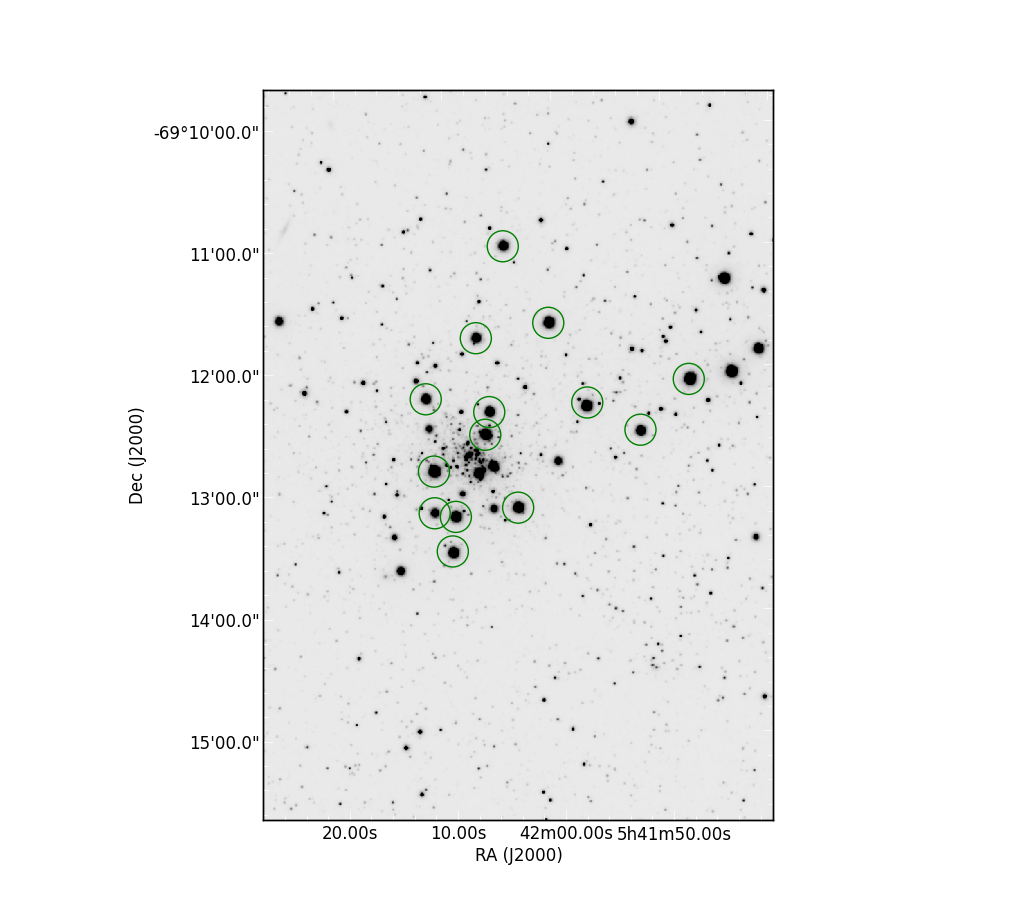
\includegraphics[width=9.0cm]{NGC2100-targets}
 \caption{Positions of the NGC\,2100 KMOS targets overlaid on a VISTA $J$-band image.
          Green circles indicate KMOS targets.
          The adopted cluster centre has been marked by a blue cross.\label{fig:targets}
          }
\end{figure}

% subsection target_selection (end)
\subsection{KMOS Observations} % (fold)
\label{sub:kmos_observations}

% subsection kmos_observations (end)
These observations were obtained as part of the KMOS Guaranteed Time Observing (PI: Evans 095.B-0022) and were conducted in March 2015.
The observations consisted of $8\times10$\,s exposures taken with the YJ grating with sky offset exposures (S) interleaved between the object (O) exposures in an O,~S,~O observing pattern.
In addition, a standard set of KMOS calibration frames were obtained as well as observations of HD\,51506 (B5) as the telluric standard star.
Seeing conditions were stable at $\sim$1.0\,arcseconds for the course of the observations.

The KMOS/esorex standard routines~\citep[SPARK;][]{2013A&A...558A..56D} were used to calibrate and reconstruct the data cubes.
Telluric correction was performed using the 24-arm telluric correction routine where the methodology is described in detail by
~\citet{2015ApJ...803...14P}.
Briefly, corrections to the standard telluric recipe are put in place to correct for slight differences in wavelength calibration between the telluric and science spectra.
This is implemented using an iterative cross-correlation approach.
Additionally, differences in the strength of the telluric features are corrected by applying a simple scaling using the equation,

\begin{equation}
  T_{2} = (T_{1} + c) / (1 + c)
\end{equation}

\noindent where $T_{2}$ is the scaled telluric-standard spectrum, $T_{1}$ is the uncorrected telluric-standard spectrum and $c$ is the scaling parameter which is varied from $c~=~-0.5$ to $c~=~0.5$ in increments of 0.02.
The best $c$ value is chosen based on the overall standard deviation of the spectrum, i.e. the $c$ value producing the smallest $\sigma$ is selected.
Once these corrections are accounted for, the science spectra are divided by the appropriate telluric spectrum for that particular IFU.


\begin{table*}
\caption{
        Summary of VLT-KMOS targets in NGC\,2100.\label{tb:obs-params}
        }
\scriptsize
\begin{center}
\begin{tabular}{lrcccccccccl}
 \hline
 \hline
ID & S/N & $\alpha$ (J2000) & $\delta$ (J2000) & $B$ & $V$ & $I$ & $J$ & $H$ & $K_{\rm s}$ & RV (\kms) & Notes \\
 \hline
J054147.86-691205.9 & 318 & 05:41:47.873 & -69:12:05.959 & 16.488 & 13.749 &  9.769 &  9.525 &  8.603 & 8.200 &  250.3 $\pm$4.7\\
J054152.51-691230.8 & 198 & 05:41:52.430 & -69:12:30.410 & 16.430 & 14.267 & 11.970 & 10.413 &  9.526 & 9.155 &  249.3 $\pm$2.6\\
J054157.44-691218.1 & 202 & 05:41:57.286 & -69:12:16.480 & 14.074 & 13.019 & 11.170 &  9.811 &  9.036 & 8.738 &  245.6 $\pm$3.5 & C2\\
J054203.90-691307.4 & 252 & 05:42:03.877 & -69:13:07.410 & 15.624 & 13.579 & 11.410 &  9.839 &  8.996 & 8.740 &  251.1 $\pm$2.8\\
J054206.36-691220.2 & 196 & 05:42:06.348 & -69:12:20.150 &$\ldots$&$\ldots$& 11.810 & 10.371 &  9.480 & 9.159 &  255.7 $\pm$4.9 & B17\\
J054206.77-691231.1 & 256 & 05:42:06.764 & -69:12:31.245 & 15.643 & 13.675 & 11.390 &  9.977 &  9.150 & 8.807 &  250.6 $\pm$3.4\\
J054209.66-691311.2 & 240 & 05:42:09.647 & -69:13:11.263 & 15.367 & 13.383 & 11.370 &  9.976 &  9.136 & 8.841 &  254.3 $\pm$4.1\\
J054209.98-691328.8 & 250 & 05:42:10.001 & -69:13:28.210 & 16.060 & 13.827 & 11.580 & 10.021 &  9.150 & 8.823 &  250.2 $\pm$3.0 & C32\\
J054211.56-691248.7 & 304 & 05:42:11.574 & -69:12:48.770 & 16.327 & 14.033 & 11.450 &  9.557 &  8.617 & 8.264 &  255.5 $\pm$4.3\\
J054211.61-691309.2 & 151 & 05:42:11.592 & -69:13:09.257 & 16.165 & 14.272 & 12.340 & 10.943 & 10.090 & 9.788 &  256.6 $\pm$6.1\\
J054212.20-691213.3 & 195 & 05:42:12.182 & -69:12:13.144 & 15.483 & 13.606 & 11.750 & 10.440 &  9.622 & 9.335 &  260.0 $\pm$4.8\\
J054200.74-691137.0 & 262 & 05:42:00.722 & -69:11:36.925 & 15.579 & 13.674 &  9.421 &  9.900 &  9.017 & 8.683 &  248.8 $\pm$2.7\\
J054204.78-691058.8 & 211 & 05:42:04.762 & -69:10:58.816 & 15.550 & 13.800 & 12.770 & 10.319 &  9.427 & 9.159 &  256.1 $\pm$4.0\\
J054207.45-691143.8 & 201 & 05:42:07.435 & -69:11:43.692 & 15.531 & 13.661 & 11.780 & 10.482 &  9.610 & 9.351 &  252.5 $\pm$3.0\\



% J054147.86-691205.9 0207-0134568
% J054152.51-691230.8 0207-0134683
% J054157.44-691218.1 0207-0134811
% J054203.90-691307.4 0207-0134979
% J054206.36-691220.2 0207-0135059
% J054206.77-691231.1 0207-0135069
% J054209.66-691311.2 0207-0135150
% J054209.98-691328.8 0207-0135162
% J054211.56-691248.7 0207-0135205
% J054211.61-691309.2 0207-0135206
% J054212.20-691213.3 0207-0135220
% J054200.74-691137.0 0208-0135292
% J054204.78-691058.8 0208-0135383
% J054207.45-691143.8 0208-0135446
\hline
\end{tabular}
\end{center}
{Photometric data taken from the SIMBAD database. Typical errors on photometric data:
0.026, 0.014, 0.04, 0.024, 0.026, 0.022 respectively.
Near-IR data taken from 2MASS.}
\end{table*}

% section observations (end)

\section{Results} % (fold)
\label{sec:results}

% section results (end)

\subsection{Radial velocities} % (fold)
\label{sub:radial_velocities}
Radial velocities are estimated using an iterative cross-correlation method.
To ensure systematic shifts are removed, the observed spectra are first cross-correlated against a spectrum of the Earth's atmosphere, taken from the ISAAC web-pages at a much higher resolution than that of the KMOS observations.
This spectrum is then degraded to the resolution of the observations using a simple Gaussian filter.
The cross-correlation is performed within the $1.140-1.155\,\mu$m region as a strong set of reliable telluric features dominates this region, with minimal contamination from stellar features.
The shift arising from this region is typically between $0-10\,$\kms and is then applied to the $1.16-1.22\,\mu$m region, i.e. where the radial velocity is estimated.

Once the observed spectra are on a consistent wavelength solution, an initial guess of the radial velocity is estimated by cross-correlating the science spectra with an appropriate synthetic RSG spectrum in the $1.16-1.22\,\mu$m region.
This wavelength regime is selected based on the dominance of atomic features in the RSG spectrum at these wavelengths.
To increase reliability, this initial guess is improved upon by using seven, independent, carefully selected strong stellar absorption lines which are chosen based on the strength of the line and the level of telluric contamination.
% Figure~\ref{fig:rv-regions} illustrates the selected features used for the analysis.

Radial velocities are independently calculated for each line using again the iterative cross-correlation method.
This results in seven estimates of the radial velocity for each star which are then compared.
Any line which produces a radial velocity which is an obvious outlier to the distribution is rejected (i.e. several ten \kms discrepant from any other value).
This can occasionally be the case when the cross-correlation incorrectly centres on a different spectral line, a simple visual inspection of the resulting spectra - once the shift has been implemented - is sufficient to remove these rare cases.

The final radial velocity for each star is the mean of the distribution resulting from the (non-rejected) lines,
where the error on this mean is calculated by taking the standard deviation of the data, normalised by the number of regions used ($err~=~\sigma/N_{regions}$).
This method is known to work well for KMOS spectra~\citep{2015ApJ...798...23L,2015ApJ...803...14P}.
% Not rejecting these outliers has the effect of increasing the error on each individual radial velocity but it does not alter the mean of the sample or the deviation significantly ($<RV>~=~251\pm3.4\,$\kms).

Figure~\ref{fig:rvs} shows all stellar radial velocity estimates as a function of distance from the centre of the cluster, alongside the systemic radial velocity of the LMC (green dashed line).
Given the low dispersion of the radial velocity measurements for the KMOS targets, we confirm that all of the targets within this sample are members of NGC\,2100.
The average value of the sample is $251.5\pm3.4\,$\kms.
Below, this average value is compared with previous measurements within the cluster and
Table~\ref{tb:rvs} details these previous measurements.

Recently,~\cite{2015arXiv150803490E} used AAOmega to measure radial velocities of massive stars within the LMC, which included two sources in NGC\,2100: stars 407 (O9.5\,II $258.5\pm3.4$\,\kms) and 408 (B3\,Ia; $250.6\pm1.3$\,\kms).
Massive blue stars are known to preferentially reside within binary systems~\citep{2012Sci...337..444S} which could increase the measured radial velocities significantly~\citep{2012A&A...546A..73H}.
If these massive blue stars were in binaries we would expect the RSG radial velocities to be lower than the velocities measured in these stars.
We find however, good agreement between our measurements and those from~\cite{2015arXiv150803490E}, indicating that these two blue stars within NGC\,2100 are not affected significantly by the effects of binary motions.


\citet[henceforth JT94]{1994A&A...282..717J} measured radial velocities for four RSGs in NGC\,2100~\citep[B17, C2, C32 and C34, using the nomenclature of][]{1974A&AS...15..261R}.
Three of these stars have been observed with KMOS in the present study (J054206.36-691220.2; B17, J054157.44-691218.1; C2 and J054209.98-691328.8; C32).
The average offset between these stars which are common to the samples is $-11.2\pm9.0$\,\kms, dominated by the difference the in measurements of C2.
However, when taken in context with other measurements in NGC\,2100 the value of $270\pm8\,$\kms appears to be a low-significance outlier.


\cite{1983ApJ...272..488F} compiled integrated-light radial velocities from~\cite{1972MNRAS.159..445A} and
\cite{1970PhD...........F} to define an average of $267\pm13\,$\kms for NGC\,2100.
Whereas~\cite{1971ApJ...169..271S}, measured the radial velocity of the HII gas of NGC\,2100 as $282.2\pm2.5\,$\kms.

We conclude that there exists no significant offset between our measurements and previous estimates within NGC\,2100.
Another confirmation that absolute radial velocities can be precisely measured with KMOS spectra.

% \begin{figure*}
%  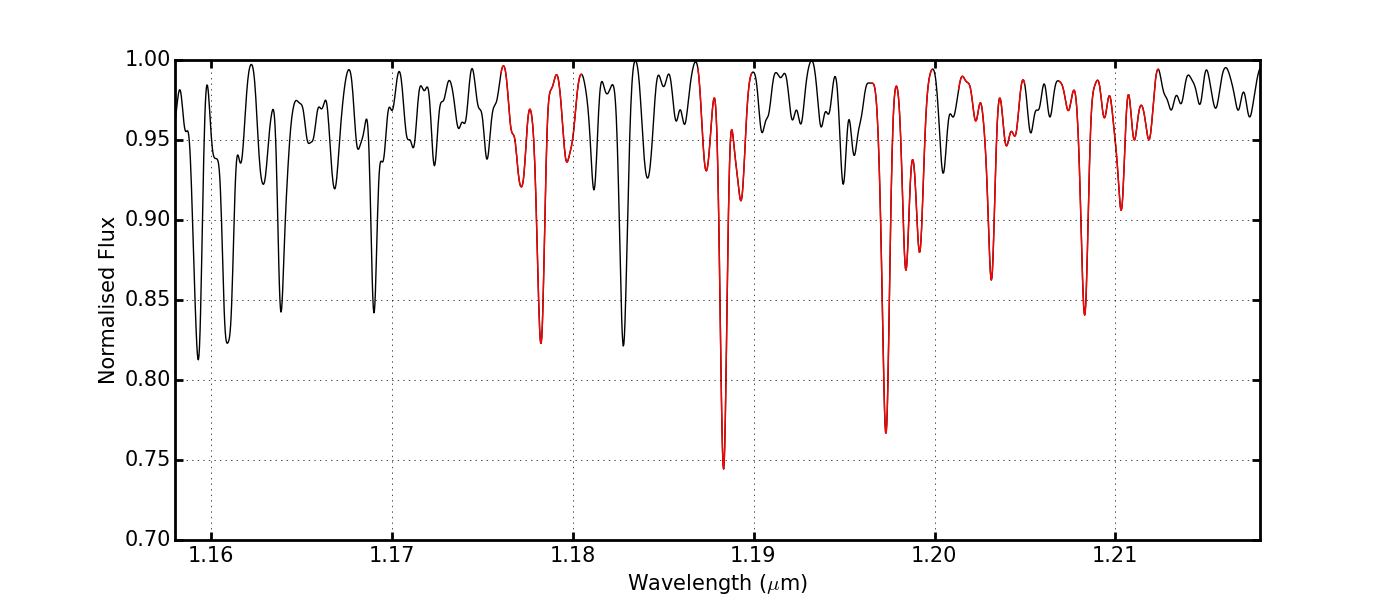
\includegraphics[width=18.0cm]{NGC2100-rv-regions}
%  \caption{Synthetic RSG spectrum used calculate the radial velocities for programme stars.
%  Red regions illustrate those used to cross-correlate the observed spectra with this synthetic spectrum.
%  These regions provide consistent results with an average dispersion between the five regions of of 2.3\,\kms.
% \label{fig:rv-regions}
%           }
% \end{figure*}


\begin{figure}
 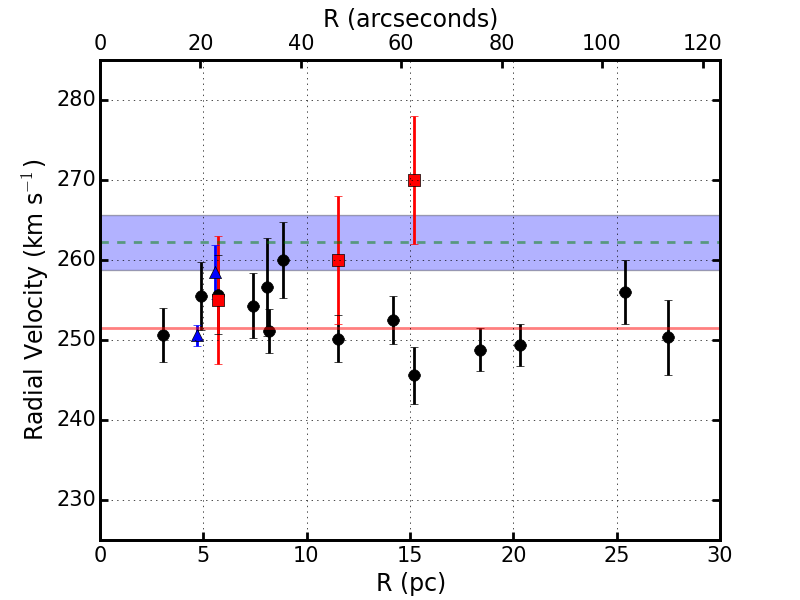
\includegraphics[width=9.0cm]{NGC2100-rv-v8}
 \caption{Radial velocities of KMOS targets shown as a function of distance from the cluster centre.
 Green dashed line shows the LMC systemic velocity with the error highlighted by the blue shaded region
 {\citep[$262.2\pm3.4$\,\kms;][]{2012AJ....144....4M}}
 The solid red line shows the mean of the sample ($251.5\pm3.4\,$\kms).
 Blue triangles show the two young stars studied in~\protect\cite{2015arXiv150803490E} and red squares show previous estimates for three of the targets
 {\citep{1994A&A...282..717J}}.\label{fig:rvs}}
\end{figure}

\begin{table*}
\begin{center}
\caption{
        Literature radial velocity measurements for NGC\,2100.\label{tb:rvs}
        }
\scriptsize
\begin{threeparttable}
\begin{tabular}{lcccll}
 \hline
 \hline
\multicolumn{2}{c}{ID} & \multicolumn{2}{c}{RV (\kms)}  & Reference & Notes \\
Lit. & current study & Lit. & current study\\
 \hline
407 & ---         & $258.5\pm3.4$     & \ldots        & \cite{2015arXiv150803490E} &  O9.5\,II  \\
408 & ---         & $250.6\pm1.3$     & \ldots        & \cite{2015arXiv150803490E} &  B3\,Ia    \\
B17 & J054206.36-691220.2 & $255\pm8$ & $255.7\pm4.9$ & {\cite{1994A&A...282..717J}} \\
C2  & J054157.44-691218.1 & $270\pm8$ & $245.6\pm3.5$ & {\cite{1994A&A...282..717J}} \\
C32 & J054209.98-691328.8 & $260\pm8$ & $250.2\pm3.0$ & {\cite{1994A&A...282..717J}} \\
C34 & ---         & $265\pm8$         & \ldots        & {\cite{1994A&A...282..717J}} & \\
NGC\,2100 & ---   & $280\pm10(16)$    & \ldots        & {\cite{1972MNRAS.159..445A}} & Whole cluster\\
NGC\,2100 & --- & $282.2\pm2.5$       & \ldots        & {\cite{1971ApJ...169..271S}} & Gas\\
NGC\,2100 & --- & $253\pm17$          & \ldots        & {\cite{1970PhD...........F}} & \\

\hline
\end{tabular}

\begin{tablenotes}
\item Value in braces is the error defined from~\cite{1983ApJ...272..488F}.
ID and RV columns, first value is from the literature and the second is from the current study.
\end{tablenotes}
\end{threeparttable}
\end{center}
\end{table*}

\subsection{Velocity Dispersion} % (fold)
\label{sub:velocity_dispersion}

An upper limit to the line-of-sight velocity dispersion ($\sigma_{1D}$) is calculated using the equations,
\begin{equation}
  \mu = \frac{1}{\sum_{i} 1/\sigma_{i}^{2}} \sum_{i} \frac{RV_{i}}{\sigma_{i}},
\end{equation}

\begin{equation}
Var = \frac{1}{\sum_{i}1/\sigma_{i}^{2}} \sum_{i}\frac{(RV_{i} - \mu)^{2}}{\sigma_{i}^{2}},
\end{equation}

\begin{equation}
  \sigma_{1D} = \sqrt{Var \frac{N}{N - 1}},
\end{equation}

\noindent where $\sigma_{i}$ is the uncertainty on the radial velocity measurement $RV_{i}$, $\mu$ is the weighted mean and $N$ is the number of stars in the sample.
Figure~\ref{fig:sig1d} shows the line-of-sight velocity dispersion profile for RSGs in NGC\,2100,
where $\sigma_{1D}$ is calculated for each star using all stars closer to the cluster centre than the star in question.
The uncertainties in this figure are defined as the standard deviation of the radial velocities within the given distance, normalised by the number of measurements in the sample.
We see that the dispersion is consistent with a flat profile with a value of $\sim$3.5\,\kms.
The scatter within $10\,$pc could be owing to the low number statistics within these radii.
% Thus, we adopt $\sigma_{1D}~=~3.4\pm0.5\,$\kms, where this uncertainty is the average of all the $\sigma_{1D}$ measurements in Figure~\ref{fig:sig1d}, as an upper limit on the line-of-sight velocity dispersion profile of NGC\,2100.
A discussion on how binarity affects this distribution is given in Section~\ref{sub:velocity_dispersion_Mdyn}.


\begin{figure}
 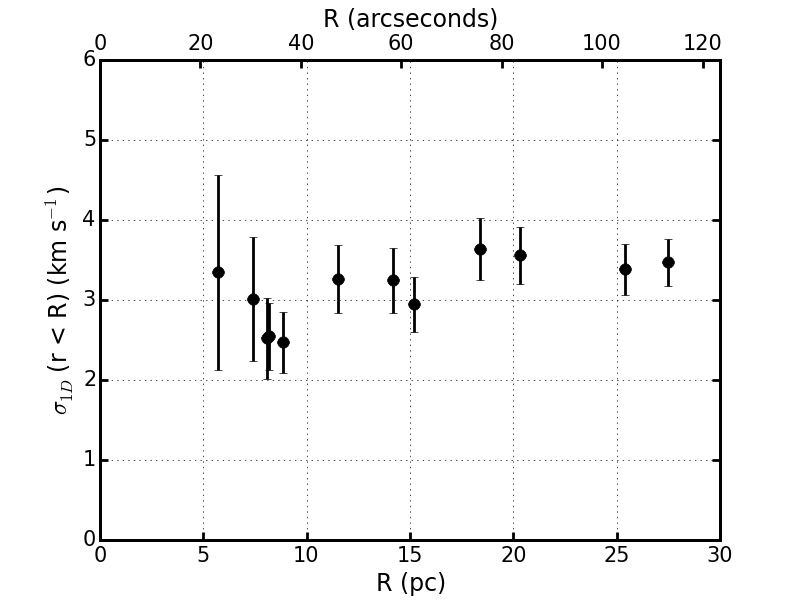
\includegraphics[width=9.0cm]{NGC2100-sig1d-v8}
 \caption{Observed line-of-sight velocity dispersion as a function of the distance from the centre of NGC\,2100.
 The measurement of $\sigma_{1D}$ includes the radial velocities of all RSGs internal to the target in question.
 The average $\sigma_{1D}$ from this figure is $3.4\pm0.4\,$\kms.
\label{fig:sig1d}
          }
\end{figure}


To estimate the contribution of measurement errors we performed a Monte Carlo simulation.
For each radial velocity measurement we drew random samples from a normal distribution centred on zero with a standard deviation matching that of the error on the radial velocity measurement.
Using this generated set of data the line-of-sight velocity dispersion was computed for the whole sample (as we found no evidence for variations in $\sigma_{1D}$).
This procedure was then repeated 10\,000 times and the resulting distribution is shown in Figure~\ref{fig:errs}.
From this figure we can see that the contribution of the measurement errors in comparable to the adopted $\sigma_{1D}$ for the cluster.
Therefore, using the data available we conclude that $\sigma_{1D} < 3.3\pm0.7$\kms for NGC\,2100.


% \textbf{Ben's comment:\\Did you subtract the measurement error in quadrature first? If you had an intrinsic sigma of zero, but an average error per measurement of e.g. 5kms, then the velocity dispersion you would measure would be $\sim$5kms and would be dominated by your instrumental errors. To find the `real' sigma, you need to subtract the measurement error in quadrature. }


\begin{figure}
 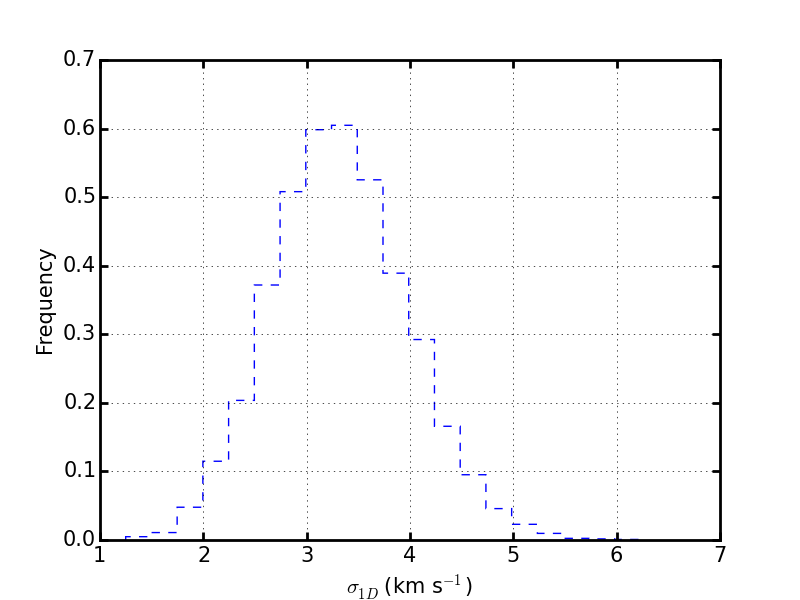
\includegraphics[width=9.0cm]{NGC2100-errors}
 \caption{Contribution of measurement errors to the line-of-sight velocity dispersion profile for NGC\,2100.
 The mean value for the contribution of measurement errors is $3.3\pm0.7\,$\kms.
\label{fig:errs}
          }
\end{figure}


% subsection velocity_dispersion (end)

\subsection{Dynamical Mass} % (fold)
\label{sub:dynamical_mass}


Using $\sigma_{1D}$ as an upper limit on the velocity distribution, one can calculate the dynamical mass of the cluster using the virial equation,

\begin{equation}
  M_{dyn} = \frac{\eta\sigma_{1D}^{2}r_{eff}}{G},
  \label{eq:vir}
\end{equation}

\noindent where $M_{dyn}$ is the dynamical mass, $\eta~=~6r_{vir}/r_{eff}~=~9.75$ providing the density profile of the cluster is sufficiently steep~\citep{2010ARA&A..48..431P}.
However, NGC\,2100 has a relatively shallow density profile~\citep[$\gamma~=~2.44\pm0.14$;][]{2003MNRAS.338...85M} which means $\eta<9.75$ and therefore the estimate of $M_{dyn}$ is knowingly an upper limit.
Using $\sigma_{1D}~=~3.3\pm0.7$\,\kms and equation~\ref{eq:vir}, the dynamical mass of NGC\,2100 is $M_{dyn}~=~(11.2\pm4.4)\times 10^{4}M_{\odot}$.
Comparing this to the photometric mass $M_{phot}~=~(2.3\pm1.0)\times 10^{4}M_{\odot}$~\citep{2005ApJS..161..304M} we see that the dynamical mass is significantly larger.
\citet{2010MNRAS.402.1750G} explain this discrepancy by demonstrating that binary motions can increase the measured velocity dispersion profile.
\citet{2012A&A...546A..73H} noted that had binarity been neglected they would have measured a $\sigma_{1D}$ a factor of five higher for R136.
% is larger, which is expected owing to binary motions within the cluster~\citep{2010MNRAS.402.1750G}.
However, the mean lifetime for RSGs within binary systems is significantly decreased and where mass transfer occurs, the number of RSGs drastically decreases~\citep{2008MNRAS.384.1109E}.
We can therefore expect that the numbers of RSGs in close binary systems are very small~\citep{2009ApJ...696.2014D}.
The fraction of RSGs in longer period binary systems is more uncertain, however, these systems would increase the line-of-sight velocity dispersion to a lesser degree.

Assuming that the population of RSGs we observe is entirely single leads to the conclusion that the only factor affecting the estimation of $M_{dyn}$ is the $\eta$ parameter.
Using a lower estimate of $\eta~=~7.0$~\citep[estimated from Fig. 4a in][ giving $M_{dyn}~=~(8.0\pm3.1)\times 10^{4}M_{\odot}$]{2010ARA&A..48..431P}, cannot account for the discrepancy between the measured masses.
However, if the measured line-of-sight velocity dispersion is inflated by binary motions, as discussed in Section~\ref{sub:velocity_dispersion_Mdyn}, the measured dynamical mass would be correspondingly increased.

% which accounts for the discrepancy between the measured masses.
% As we can account for the differences in the mass measurements using just the $\eta$ parameter, this implies that the assumption that the RSGs in our sample are single objects is correct.

% subsection dynamical_mass (end)


% section radial_velocities (end)

\subsection{Stellar Parameters} % (fold)
\label{sub:stellar_parameters}

Stellar parameters are estimated using the $J$-band analysis technique described initially in~\cite{2010MNRAS.407.1203D}
and tested rigorously by~\cite{2014ApJ...788...58G} and~\cite{2015ApJ...806...21D}.
These studies show that using a narrow spectral window within the $J$-band one can accurately derive overall metallicities ([Z]) to better than
$\pm0.15\,dex$ at the resolution of KMOS observations with S/N~$\ge~100$.
\cite{2015ApJ...803...14P} built on this by demonstrating the feasibility of this technique using KMOS spectra.

The analysis uses synthetic RSG spectra, extracted from {\sc marcs} model atmospheres~\citep{2008A&A...486..951G},
computed with corrections for non-local thermodynamic equilibrium for stellar lines from titanium, iron, silicon and magnesium
\citep{2012ApJ...751..156B,2013ApJ...764..115B,2015ApJ...804..113B}.
The parameter ranges for the grid of synthetic RSG spectra are listed in Table~\ref{tb:mod_range}.
The synthetic spectra are compared with observations using a $\chi$-squared minimisation approach where the synthetic spectra are degraded to the resolution and sampling of the observations.

Estimated stellar parameters are listed in Table~\ref{tb:stellar-params}.
Reliable parameters could not be estimated for two stars (J054206.36-691220.2 and J054211.61-691309.2).
These two stars are rejected from further analysis.
Figure~\ref{fig:model_fits} shows the observed KMOS spectra (black) along with each best-fitting model spectrum (red).
The average metallicity for the 12 stars within the NGC\,2100 sample is $-0.39\pm0.10\,dex$.

The average metallicity in NGC\,2100 compares well with estimates of the cluster metallicity using isochrone fitting to the optical colour-magnitude diagram~\citep[$-0.34\,dex$;][]{2015A&A...575A..62N}.
JT94 reported the only other estimate of stellar metallicity within this cluster,
who estimated metallicities using optical spectroscopy of four RSGs.
These authors found an average metallicity for NGC\,2100 of $-0.32\pm0.03\,dex$, which our estimate agrees well with.
We find that there are three targets in common with our study: B17, C2, C32~\citep[using the][nomenclature]{1974A&AS...15..261R}.
Comparing results we find B17 (J054206.36-691220.2) does not have reliable stellar parameters. Currently, we have no explanation for why this is the case.

% has a spuriously high  metallicity for the sample.
% However, this spectrum displays no obvious features of a poor telluric correction or sky subtraction with a signal-to-noise ratio far exceeding that of our minimum threshold to perform the analysis.

The results for C2 (J054157.44-691218.1) are consistent with what is reported in JT94, although we note that surface gravity reported here agrees with the estimated photometric surface gravity and the spectroscopic surface gravity in JT94 is significantly lower.
In addition we note that the microturblence value quoted in the current study is on the edge of the allowed model grid.
The results for C32 (J054209.98-691328.8) are consistent with what is reported in JT94, although we note that the best fit microturblence value is also at the edge of the model grid.


Using the same analysis technique as in this study,
\cite{2015ApJ...806...21D} estimate metallicities for nine RSGs within the LMC,
finding an average value of $-0.37\pm0.14\,dex$ which our estimate agrees well with.
In Figure~\ref{fig:TeffvsZ} we compare the effective temperatures and metallicities from NGC\,2100 with those derived for RSGs elsewhere in the LMC.
We find excellent agreement in the distribution of temperatures from the two studies, with the average agreeing well.
The range in [Z] from the LMC population is slightly larger than that of the NGC\,2100 RSGs, which is expected when comparing a star cluster with an entire galaxy, however the averages for the two studies agree very well.


\begin{figure}
 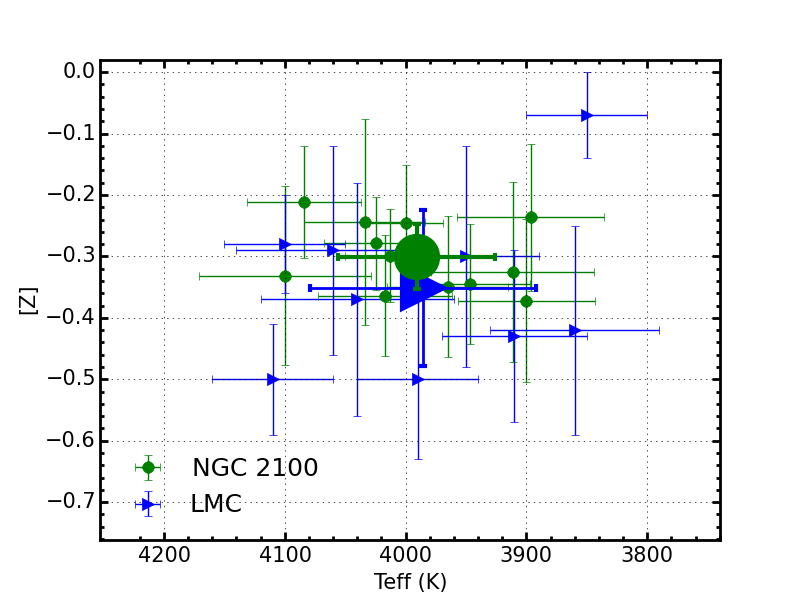
\includegraphics[width=9.0cm]{NGC2100-TeffvsZ-2100-LMC}
 \caption{Estimated metallicities for NGC\,2100 RSGs in this study shown against effective temperature (green dots).
        For comparison we show the distribution of LMC RSGs in~\citet[blue triangles][]{2015ApJ...806...21D}.
        This demonstrates the remarkable agreement between the effective temperature ranges and averages for RSGs within these two samples.
\label{fig:TeffvsZ}
          }
\end{figure}

\begin{figure*}
 %\vspace{302pt}
 \begin{center}
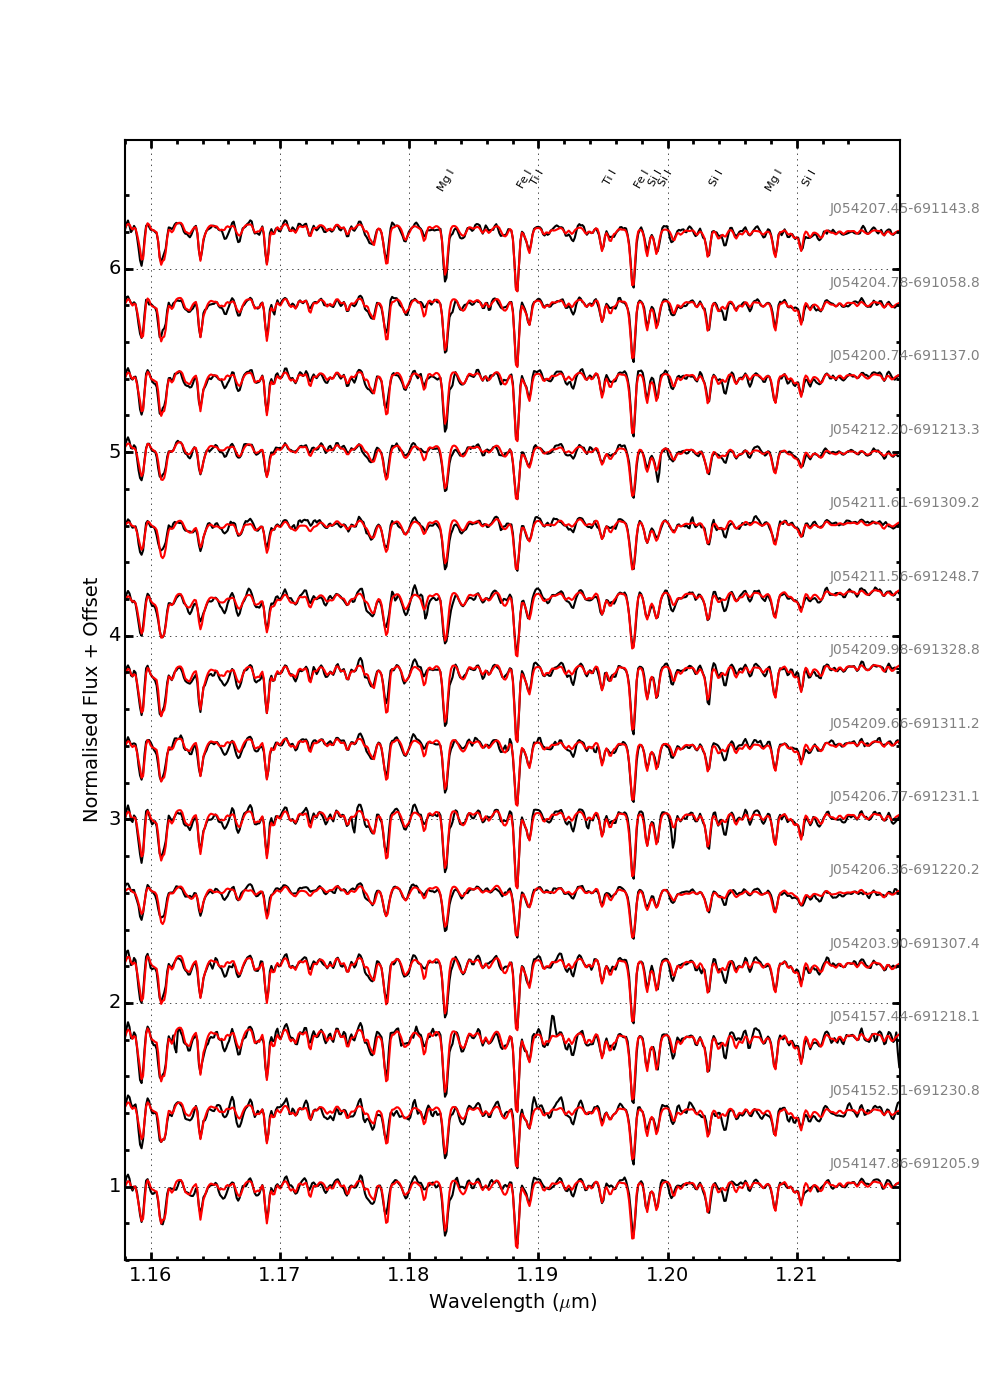
\includegraphics[width=16cm]{NGC2100-model-fits}
\caption{KMOS spectra of the NGC\,2100 RSGs and their associated best-fit model spectra
(black and red lines, respectively).
The lines used for the analysis from left-to-right by species are:
Fe\,I$\lambda\lambda$1.188285,
1.197305,
Mg\,I$\lambda\lambda$1.182819,
1.208335,
Si\,I$\lambda\lambda$1.198419,
1.199157,
1.203151,
1.210353,
Ti\,I$\lambda\lambda$1.189289,
1.194954.
         }
\label{fig:model_fits}
\end{center}
\end{figure*}




% \begin{figure}
%  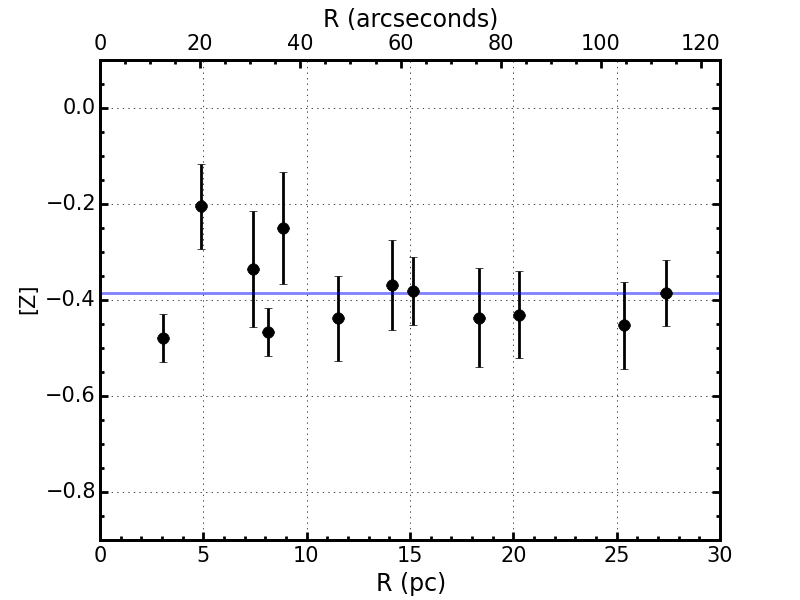
\includegraphics[width=9.0cm]{NGC2100-ZvsR}
%  \caption{Estimated metallicities shown against distance from the centre of the cluster where the solid blue line denotes the mean of the sample $-0.39\pm0.10\,dex$.
% \label{fig:ZvsR}
%           }
% \end{figure}

\begin{table}
\caption{
Model grid used for analysis.\label{tb:mod_range}
         }
\scriptsize
\begin{center}
\begin{tabular}{lccc}
 \hline
 \hline
  Model Parameter & Min. & Max. & Step size \\
 \hline
T$_{eff}$ (K)        & 3400 & 4400 & 100 \\
$[$Z$]$ (dex)   & $-$1.0\o & 1.0\o  & 0.1\o\\
log\,$g$ (cgs)  & $-$1.00 & 1.00 & 0.25\\
 $\xi$ (\kms)  & \pp1.0\o & 5.0\o & 0.2\o\\
 \hline
\end{tabular}
\end{center}
\end{table}

\begin{table*}
\begin{center}
\caption{
Physical parameters for the NGC\,2100 KMOS targets
\label{tb:stellar-params}
         }
\scriptsize
\begin{threeparttable}
\begin{tabular}{lc ccccc}
 \hline
 \hline
  Target  & IFU & $\xi$ (\kms) & [Z] & log\,$g$ & T$_{eff}$ (K) & Notes\\
  \hline
J054147.86-691205.9 & 7  & 3.6 $\pm$ 0.19 & -0.39 $\pm$ 0.07 &  0.12 $\pm$ 0.12 & 4048 $\pm$ 63 & \\
J054152.51-691230.8 & 9  & 3.5 $\pm$ 0.18 & -0.439$\pm$ 0.09 &  0.42 $\pm$ 0.18 & 4002 $\pm$ 26 & \\
J054157.44-691218.1 & 6  & 5.0 $\pm$ 0.10 & -0.38 $\pm$ 0.07 &  0.18 $\pm$ 0.13 & 3994 $\pm$ 43 & C2\\
J054203.90-691307.4 & 12 & 4.6 $\pm$ 0.14 & -0.47 $\pm$ 0.05 &  0.24 $\pm$ 0.13 & 3894 $\pm$ 50 & \\
J054206.36-691220.2 & 24 & 2.5 $\pm$ 0.47 &  0.01 $\pm$ 0.27 &  0.45 $\pm$ 0.11 & 3773 $\pm$ 132 & B17\\
J054206.77-691231.1 & 10 & 5.0 $\pm$ 0.10 & -0.48 $\pm$ 0.05 &  0.24 $\pm$ 0.13 & 3904 $\pm$ 50 & \\
J054209.66-691311.2 & 14 & 3.7 $\pm$ 0.20 & -0.34 $\pm$ 0.12 &  0.06 $\pm$ 0.21 & 3767 $\pm$ 73 & \\
J054209.98-691328.8 & 11 & 5.0 $\pm$ 0.10 & -0.44 $\pm$ 0.09 &  0.16 $\pm$ 0.20 & 3948 $\pm$ 44 & C32\\
J054211.56-691248.7 & 20 & 3.8 $\pm$ 0.19 & -0.21 $\pm$ 0.09 & -0.01 $\pm$ 0.17 & 3906 $\pm$ 68 & \\
J054211.61-691309.2 & 18 & 2.1 $\pm$ 0.24 &  0.34 $\pm$ 0.08 &  0.75 $\pm$ 0.13 & 3800 $\pm$ 50 & \\
J054212.20-691213.3 & 22 & 3.3 $\pm$ 0.21 & -0.25 $\pm$ 0.12 &  0.36 $\pm$ 0.25 & 4040 $\pm$ 54 & \\
J054200.74-691137.0 & 4  & 4.2 $\pm$ 0.23 & -0.44 $\pm$ 0.10 &  0.17 $\pm$ 0.10 & 3784 $\pm$ 76 & \\
J054204.78-691058.8 & 3  & 4.1 $\pm$ 0.20 & -0.45 $\pm$ 0.09 &  0.48 $\pm$ 0.10 & 3893 $\pm$ 50 & \\
J054207.45-691143.8 & 2  & 4.0 $\pm$ 0.21 & -0.37 $\pm$ 0.09 &  0.48 $\pm$ 0.13 & 3864 $\pm$ 50 & \\
\\
NGC\,2100 average      & & 4.1 $\pm$ 0.58 & -0.39 $\pm$ 0.08 &  0.24 $\pm$ 0.15 & 3903 $\pm$ 87 &\\

  \hline
  \end{tabular}
\begin{tablenotes}
    \item Note: The names B17, C2 and C32 refer to~{\protect\citet{1974A&AS...15..261R}}.
\end{tablenotes}
  \end{threeparttable}
  \end{center}
\end{table*}

% section stellar_parameters (end)

\section{Discussion} % (fold)
\label{sec:discussion}

\subsection{Stellar Parameters} % (fold)
\label{sub:stellar_parameters_disc}

Luminosities have been estimated using the bolometric correction in~\cite{2013ApJ...767....3D} and a H-R diagram for the clusters is presented in Figure~\ref{fig:HRD}.
Overlaid on this H-R diagram are {\sc syclist} stellar isochrones for SMC-like~\citep[solid lines,][]{2013A&A...558A.103G} and Solar-like~\citep[dashed lines,][]{2012A&A...537A.146E} models, where stellar rotation is 40\% of break-up velocity.
Even though the temperatures covered by the SMC-like models do not accurately represent the distribution of temperatures observed in this study, it remains useful to fit the data using these models to estimate an age for NGC\,2100.
The Solar-like models (dashed) demonstrate that increasing the metallicity of the sample
a) decreases the temperatures of the RSGs~\citep[something which is not observed by][]{2015ApJ...803...14P},
b) induces a blue-ward evolution for the youngest models and
c) decreases the luminosity for the oldest models.


% The narrow range in masses implied by the luminosities of the stars (regardless of which evolutionary models is used) adds strength to the argument that these stars were all formed in a single burst of star formation.

\begin{figure}
 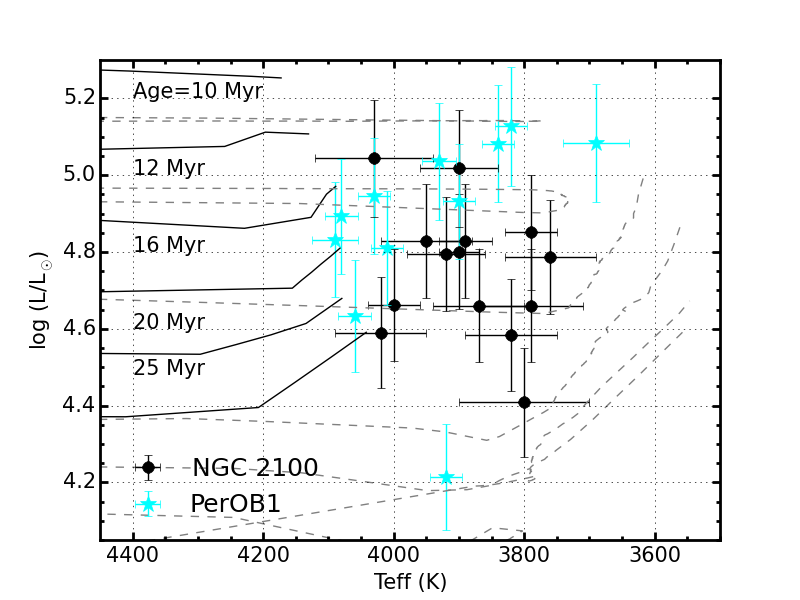
\includegraphics[width=9.0cm]{NGC2100-HRD-perOB1}
 \caption{H-R diagram for 12 RSGs in NGC2100.
  % Bolometric corrections computed using~\citet{2013ApJ...767....3D}.
  Cluster isochrones for solar~\citep[dashed lines;][]{2012A&A...537A.146E} and SMC-like~\citep[solid lines;][]{2013A&A...558A.103G} metal abundances,
  where stellar rotation is 40\% of the break-up velocity, are shown for ages of 10-32\,Myr. For comparison, 11 RSGs from the Galactic YMC Perseus OB-1 are overlaid~\citep{2014ApJ...788...58G}.\label{fig:HRD}
          }
\end{figure}

In addition, in Figure~\ref{fig:HRD}, 11 RSGs from the Galactic star cluster Perseus OB-1~\citep[PerOB1;][]{2014ApJ...787..142G} are overlaid with blue stars, where stellar parameters are estimated using the same analysis technique as in this study.
PerOB1 is a star cluster with similar mass and age~\citep[$2\times10^{4}\,$M$_{\odot}$ and 14\,Myr respectively;][]{2010ApJS..186..191C} to NGC\,2100 and a comparison between the stellar components of these two clusters using a consistent analysis technique is useful to highlight differences in stellar evolution within clusters at different metallicities.

We can see from Figure~\ref{fig:HRD} that generally, the two data sets are in good agreement.
The median luminosity for the PerOB1 targets ($10^{4.93\pm0.15}\,$L$_{\odot}$) is slightly above that of NGC\,2100 ($10^{4.77\pm0.15}\,$L$_{\odot}$) which could represent the slight difference in the ages of the two clusters.
As PerOB1 is younger, the average mass for a RSG in the cluster will be larger than the average in NGC\,2100.
Therefore we would expect to see higher luminosity RSGs in PerOB1.
However, the difference between the two samples is barely significant and is consistent with a constant luminosity.
The average effective temperature of the two data sets is consistent between the two samples.
As~\cite{2015ApJ...803...14P} point out, this is not predicted by evolutionary models.
Overall, by comparing these two star clusters with a similar mass, age and stellar population we conclude that there exists no significant difference in appearance on the H-R diagram of RSGs within star clusters of different metallicities.




% \begin{figure}
%  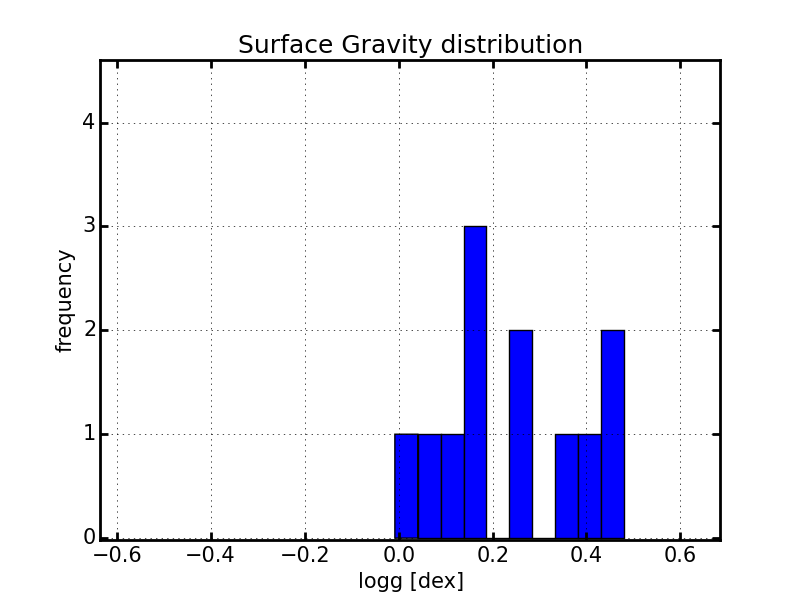
\includegraphics[width=9.0cm]{NGC2100-logg-dist-v6}
%  \caption{Histogram showing the range of surface gravities estimated. Average value $0.24\pm0.15\,dex$.
%  For Illustration only.\label{fig:loggdist}
%           }
% \end{figure}



% subsection stellar_parameters (end)
\subsection{Velocity Dispersion and Dynamical Mass} % (fold)
\label{sub:velocity_dispersion_Mdyn}

This study represents the first estimate of the line-of-sight velocity dispersion profile for NGC\,2100.
Comparing this estimate with that of other YMCs in the Local Universe is useful to ascertain whether this cluster shares similar properties to other more well studied YMCs.
We find the dynamical properties NGC\,2100 are well matched by other clusters with similar masses and ages, particularly so with RSGC02, a Galactic YMC.
% Below we compare the dynamical results for NGC\,2100 to that of several young massive clusters first within the LMC and then within the Galaxy.
% A comparison with a small sample of Local Group YMCs reveals the trend that very young massive clusters have a larger line-of-sight velocity dispersion which relaxes to $\sim$3\,\kms at 10-100\,Myr.

Owing to the non-negligible contribution from measurement errors the $\sigma_{1D}$ adopted here is a upper limit to the ``true'' dispersion within the cluster.
Using the date available we can rule out a $\sigma_{1D}$ value significantly larger than $3.3\pm0.7\,$\kms and the dispersion we measure is consistent with zero dispersion within the cluster.

By extension, the dynamical mass estimated here is therefore also an upper limit to the ``true'' mass of the cluster.
There are several factors which could alter the value of the dynamical mass estimate.
The likely values of the $\eta$ parameter are discussed in~\ref{sub:dynamical_mass} and any change in this value will act to decrease the dynamical mass measurement.
Using a lower limit of $\eta$ does not account for the discrepancy between the dynamical mass measured here and the literature photometric mass of the cluster.
However, we note that if the measured $\sigma_{1D}$ was reduced by a factor of 0.25, the calculated dynamical mass is consistent with the literature value for the photometric mass.
This factor represents a binary fraction calculated in~\citet{2010MNRAS.402.1750G}.



% \subsubsection{Comparison with LMC clusters} % (fold)
% \label{sub:comparison_with_lmc_clusters}


% The line-of-sight velocity dispersion profile of the young massive cluster R136 has been estimated at 6\,\kms~\citep{2012A&A...546A..73H} using multi-epoch spectroscopy from the VLT-Flames Tarantula Survey~\citep{2011A&A...530A.108E}.
% NGC\,2100 and R136 are both located within the 30 Doradus region and within the LMC\,2 supershell.
% R136 is around twice as massive as NGC\,2100 with the photometric mass of R136 being estimated at $\sim10^{5}M_{\odot}$ with an age less than 2\,Myr~\citep{1998ApJ...509..879D,1998ApJ...493..180M,2010MNRAS.408..731C}.
% This makes R136 significantly younger than NGC\,2100 ($\sim20$\,Myr) and it is therefore unsurprising that the velocity dispersion profile is larger for R136 as one would expect a massive cluster to relax over time.

% NGC\,1850 is a young LMC massive cluster with a photometric mass of $1.4\times10^{5}$ and a recently revised age of $93\,$Myr
% \citep{2015A&A...575A..62N}.
% \citet{2005ApJS..161..304M} report a line-of-sight velocity dispersion for this cluster as $3.0\pm0.7\,$\kms which compares well to the dispersion in NGC\,2100 even though this cluster is significantly older and more massive.

% NGC\,2004 is a young massive cluster in the LMC with a mass and age similar to that of NGC\,2100~\citep[20\,Myr; $2\times10^{4}M_{\odot}$][and references therein]{2015A&A...575A..62N}.
% \citet{2006A&A...456..623E} obtained multi-epoch spectra for massive stars within this cluster and derive radial velocities without however a dynamical analysis of the cluster.
% This cluster has remarkably similar properties to NGC\,2100 and therefore a comparison between their dynamical properties is useful to investigate the intrinsic distribution of dynamical properties within young massive clusters.
% However, this is beyond the scope of the current study.

% % subsubsection comparison_with_lmc_clusters (end)

% \subsubsection{Comparison with Galactic Clusters} % (fold)
% \label{sub:galactic_clusters}

% RSGC01 is a cluster with a large population of RSGs within the Galaxy~\citep{2007ApJ...671..781D}.
% This cluster is shown to have a mass $\sim3\times10^{4}M_{\odot}$ with an age 17\,Myr and a velocity dispersion of 2.8\,\kms.
% Therefore this cluster compares remarkably well with the properties of NGC\,2100.

% Westerlund\,1 is a massive young star cluster in the Galaxy with a large population of massive stars~\citep{2005A&A...434..949C}.
% This cluster is young compared to NGC\,2100 with an age of 3.5\,Myr therefore many of the stars which will become RSGs in the future are currently fusing hydrogen on the main sequence.
% The photometric mass of Westerlund\,1 is $\sim3\times10^{4}M_{\odot}$ with a measured velocity dispersion of 5.8\,\kms.
% Like R136 in the LMC, Westerlund\,1 has a higher velocity dispersion and a young age.

% % subsubsection galactic_clusters (end)

% subsection velocity_dispersion (end)

\subsection{Simulated Cluster Spectrum Analysis} % (fold)
\label{sub:integrated_light_cluster_analysis}

We can use the individual stars in NGC\,2100 to simulate the analysis of a YMC in the more distant Universe, using the assumption that RSGs dominate the flux from such a cluster~\citep{2013MNRAS.430L..35G}.
\cite{2014ApJ...788...58G} use this assumption to create a cluster spectrum for the Galactic star cluster Perseus OB-1 and show that by analysing the combined spectrum from 11 RSGs the resulting parameters are consistent with the average parameters estimated using the individual stars.
By reconstructing the test performed by these authors we can test how metallicity affects this analysis.
NGC\,2100 has a similar mass and age to Perseus OB-1 with and~\cite{2014ApJ...788...58G} study a similar number of RSGs to this study,
therefore a direct comparison between the two clusters is useful to study any metallicity dependence.

% NGC\,2100 has a mass $>4.6~\times~10^4M_{\odot}$, an age of $\sim20\,$Myr with a known population of RSGs and is therefore a good Local Universe analogue for more distant young massive clusters.
% Using such an analysis on a LMC-like metallicity young massive cluster allows one to simulate the conditions in the early Universe.
% demonstrate that this technique can be used to simulate observations of young massive clusters at Solar-like metallicities.

To create the ``Cluster Spectrum'' we sum all the individual RSG spectra weighted by their $J$-band luminosities.
The resulting spectrum is then degraded to the lowest resolution spectrum of the sample using a simple Gaussian filter.
Figure~\ref{fig:clusterspec} shows the resulting so called Cluster Spectrum.
This spectrum is then analysed in the same way described in Section~\ref{sub:stellar_parameters} for a single RSG.
The results of this analysis are what one would expect from KMOS observations of a more-distant YMCs where individual stars cannot be resolved.
We find a metallicity of $-0.32\pm0.11\,dex$, effective temperature of $3953\pm49\,$K, surface gravity of $0.34\pm0.23\,dex$ and a microturblence velocity of $3.8\pm0.2\,$\kms which agree well with the average of the individual RSG parameters.

\begin{figure*}
 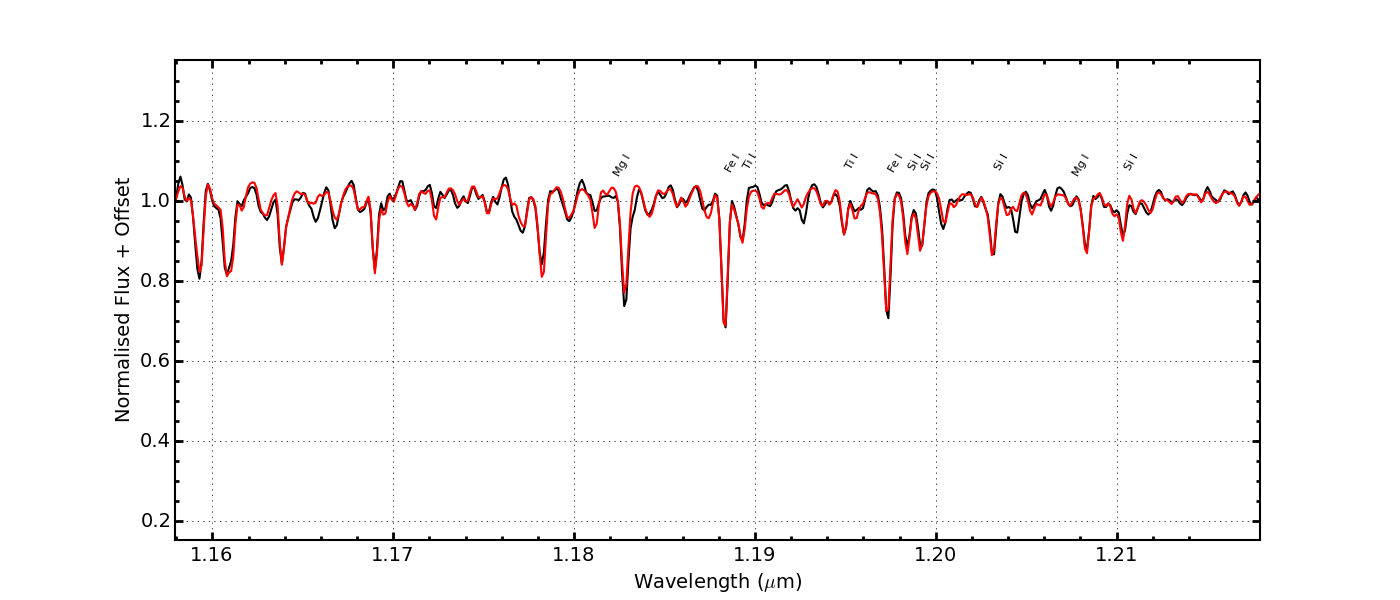
\includegraphics[width=16.0cm]{NGC2100-clusterspec}
 \caption{Combined ``Cluster Spectrum'' as a result of adding the individual RSG spectra weighted by their $J$-band luminosities. Shown in red is the best fit model spectrum.
\label{fig:clusterspec}
          }
\end{figure*}

% subsection integrated_light_cluster_analysis (end)

% section discussion (end)

\section{Conclusions} % (fold)
\label{sec:conclusions}

Using KMOS spectra of 14 RSGs in NGC\,2100 we have for the first time estimated the dynamical properties of this YMC.
Radial velocities have been estimated using KMOS, to a precision of $<~5$\,\kms, demonstrating that this instrument can be used to study the dynamical properties of star clusters in external galaxies.

The line-of-sight velocity dispersion profile has been estimated in Figure~\ref{fig:sig1d} and has been shown to be flat out to 30\,pc from the cluster centre.
An upper limit to the line-of-sight velocity dispersion of $\sigma_{1D}~<~3.3\pm0.7\,$\kms has been estimated.
We compare the line-of-sight velocity dispersion estimated here to that of other YMCs in the Local Universe and find that NGC\,2100 compares well with other massive clusters.
% This adds evidence to the theory that young star clusters appear to remain in virial equilibrium from an early age and hence expand owing to stellar evolution on a relatively slow timescale~\citep[10\,Myr][]{2010ARA&A..48..431P}.
% We compare the velocity dispersion profile estimated here to that of other young massive clusters in the LMC and the Galaxy and find that the distribution of velocity dispersions is consistent with this expansion.}

Characterisation of the velocity dispersion profile for the cluster allows for the first time the dynamical mass to be estimated (assuming virial equilibrium) as $M_{dyn}~=~(11.2\pm4.4)\times 10^{4}M_{\odot}$.
A discussion of the appropriate value of $\eta$ for this cluster is detailed in Section~\ref{sub:dynamical_mass}.
This value is shown to be significantly larger than the literature photometric mass for the cluster.

In addition to estimating the dynamical properties of NGC\,2100 we have also reliably estimated stellar parameters for 12 RSGs in NGC\,2100 using the new $J$-band analysis technique~\citep{2010MNRAS.407.1203D}.
We find the average metallicity for RSGs in NGC\,2100 is $-0.39\pm0.10\,dex$, which agrees well with previous studies within this cluster and with studies of the young stellar population of the LMC.

The H-R diagram of NGC\,2100 is compared with that of PerOB1: a Galactic YMC with a similar age, mass and stellar population.
Using stellar parameters estimated from 11 RSGs using the same analysis technique as that in this study, we demonstrate that there exists no significant difference in the appearance of the H-R diagram of YMCs between Solar- and LMC-like metallicities.

Using the H-R diagram we have estimated the age of the cluster using isochrones fitting to be $20\pm5\,$Myr, in good agreement with the estimate for this cluster from~\citet{2015A&A...575A..62N}.

By combining the individual RSG spectra within NGC\,2100, we have created an integrated ``Cluster Spectrum'' and proceeded to analyse this spectrum using the same techniques for that of the individual RSGs, as RSGs dominate the cluster light in the $J$-band~\citep{2013MNRAS.430L..35G}.
The results of this technique demonstrate the potential of this analysis for integrated light spectra of more distant YMCs in low-metallicity environments.
We find good agreement using the ``Cluster Spectrum'' with the average results of the individual RSGs.

 % and show that the estimated parameters agree well with previous studies within the LMC~\citep{2015ApJ...806...21D}.


% section conclusions (end)
\section*{Acknowledgements}

...
% \bibliographystyle{mn2e}                      % The reference style
\bibliography{journals}
% \bibliography{journals}

\begin{thebibliography}{99}

\bibitem[Andrews
\& Lloyd Evans(1972)]{1972MNRAS.159..445A} Andrews, P.~J., \& Lloyd Evans, T.\ 1972, \mnras, 159, 445

\bibitem[Banerjee
\& Kroupa(2013)]{2013ApJ...764...29B} Banerjee, S., \& Kroupa, P.\ 2013, \apj, 764, 29

\bibitem[Banerjee
\& Kroupa(2015)]{2015arXiv151203074B} Banerjee, S., \& Kroupa, P.\ 2015, arXiv:1512.03074

\bibitem[Bergemann et al.(2012)]{2012ApJ...751..156B} Bergemann, M.,
Kudritzki, R.-P., Plez, B., et al.\ 2012, \apj, 751, 156

\bibitem[Bergemann et al.(2013)]{2013ApJ...764..115B} Bergemann, M.,
Kudritzki, R.-P., W{\"u}rl, M., et al.\ 2013, \apj, 764, 115

\bibitem[Bergemann et al.(2015)]{2015ApJ...804..113B} Bergemann, M.,
Kudritzki, R.-P., Gazak, Z., Davies, B., \& Plez, B.\ 2015, \apj, 804, 113

\bibitem[Cabrera-Ziri et al.(2014)]{2014MNRAS.441.2754C} Cabrera-Ziri, I.,
Bastian, N., Davies, B., et al.\ 2014, \mnras, 441, 2754

\bibitem[Clark et
al.(2005)]{2005A&A...434..949C} Clark, J.~S., Negueruela, I., Crowther, P.~A., \& Goodwin, S.~P.\ 2005, \aap, 434, 949

\bibitem[Crowther et al.(2010)]{2010MNRAS.408..731C} Crowther, P.~A.,
Schnurr, O., Hirschi, R., et al.\ 2010, \mnras, 408, 731

\bibitem[Currie et al.(2010)]{2010ApJS..186..191C} Currie, T., Hernandez,
J., Irwin, J., et al.\ 2010, \apjs, 186, 191

\bibitem[Davies et al.(2007)]{2007ApJ...671..781D} Davies, B., Figer,
D.~F., Kudritzki, R.-P., et al.\ 2007, \apj, 671, 781

\bibitem[Davies et al.(2009)]{2009ApJ...696.2014D} Davies, B., Origlia, L.,
Kudritzki, R.-P., et al.\ 2009, \apj, 696, 2014

\bibitem[Davies et al.(2010)]{2010MNRAS.407.1203D} Davies, B., Kudritzki,
R.-P., \& Figer, D.~F.\ 2010, \mnras, 407, 1203

\bibitem[Davies et al.(2013)]{2013ApJ...767....3D} Davies, B., Kudritzki,
R.-P., Plez, B., et al.\ 2013, \apj, 767, 3

\bibitem[Davies et al.(2015)]{2015ApJ...806...21D} Davies, B., Kudritzki,
R.-P., Gazak, Z., et al.\ 2015, \apj, 806, 21

\bibitem[Davies et
al.(2013)]{2013A&A...558A..56D} Davies, R.~I., Agudo Berbel, A., Wiezorrek, E., et al.\ 2013, \aap, 558, A56

\bibitem[de Koter et al.(1998)]{1998ApJ...509..879D} de Koter, A., Heap,
S.~R., \& Hubeny, I.\ 1998, \apj, 509, 879

\bibitem[de Wit et
al.(2005)]{2005A&A...437..247D} de Wit, W.~J., Testi, L., Palla, F., \& Zinnecker, H.\ 2005, \aap, 437, 247

\bibitem[Ekstr{\"o}m et
al.(2012)]{2012A&A...537A.146E} Ekstr{\"o}m, S., Georgy, C., Eggenberger, P., et al.\ 2012, \aap, 537, A146

\bibitem[Eldridge et al.(2008)]{2008MNRAS.384.1109E} Eldridge, J.~J.,
Izzard, R.~G., \& Tout, C.~A.\ 2008, \mnras, 384, 1109

\bibitem[Elson(1991)]{1991ApJS...76..185E} Elson, R.~A.~W.\ 1991, \apjs,
76, 185

\bibitem[Evans et
al.(2006)]{2006A&A...456..623E} Evans, C.~J., Lennon, D.~J., Smartt, S.~J., \& Trundle, C.\ 2006, \aap, 456, 623

\bibitem[Evans et
al.(2011)]{2011A&A...527A..50E} Evans, C.~J., Davies, B., Kudritzki, R.-P., et al.\ 2011, \aap, 527, A50

\bibitem[Evans et
al.(2011)]{2011A&A...530A.108E} Evans, C.~J., Taylor, W.~D., H{\'e}nault-Brunet, V., et al.\ 2011, \aap, 530, A108

\bibitem[Evans et al.(2015)]{2015arXiv150803490E} Evans, C.~J., van Loon,
J.~T., Hainich, R., \& Bailey, M.\ 2015, arXiv:1508.03490

\bibitem [Ford(1970)]{1970PhD...........F} Ford, H., 1970, PhD. Thesis, University of Wisconsin.

\bibitem[Freeman et al.(1983)]{1983ApJ...272..488F} Freeman, K.~C.,
Illingworth, G., \& Oemler, A., Jr.\ 1983, \apj, 272, 488

\bibitem[Gazak et al.(2013)]{2013MNRAS.430L..35G} Gazak, J.~Z., Bastian,
N., Kudritzki, R.-P., et al.\ 2013, \mnras, 430, L35

\bibitem[Gazak et al.(2014)]{2014ApJ...788...58G} Gazak, J.~Z., Davies, B.,
Kudritzki, R., Bergemann, M., \& Plez, B.\ 2014, \apj, 788, 58

\bibitem[Gazak et al.(2014)]{2014ApJ...787..142G} Gazak, J.~Z., Davies, B.,
Bastian, N., et al.\ 2014, \apj, 787, 142

\bibitem[Gazak et al.(2015)]{2015ApJ...805..182G} Gazak, J.~Z., Kudritzki,
R., Evans, C., et al.\ 2015, \apj, 805, 182

\bibitem[Georgy et
al.(2013)]{2013A&A...558A.103G} Georgy, C., Ekstr{\"o}m, S., Eggenberger, P., et al.\ 2013, \aap, 558, A103

\bibitem[Gieles et al.(2010)]{2010MNRAS.402.1750G} Gieles, M., Sana, H.,
\& Portegies Zwart, S.~F.\ 2010, \mnras, 402, 1750

\bibitem[Gieles
\& Portegies Zwart(2011)]{2011MNRAS.410L...6G} Gieles, M., \& Portegies Zwart, S.~F.\ 2011, \mnras, 410, L6

% \bibitem[Glatt et
% al.(2010)]{2010A&A...517A..50G} Glatt, K., Grebel, E.~K., \& Koch, A.\ 2010, \aap, 517, A50
\bibitem[Gratton et
al.(2012)]{2012A&ARv..20...50G} Gratton, R.~G., Carretta, E., \& Bragaglia, A.\ 2012, \aapr, 20, 50

% \bibitem[Gratton et
% al.(2012)]{2012A&A...539A..19G} Gratton, R.~G., Lucatello, S., Carretta, E., et al.\ 2012, \aap, 539, A19

\bibitem[Gustafsson et
al.(2008)]{2008A&A...486..951G} Gustafsson, B., Edvardsson, B., Eriksson, K., et al.\ 2008, \aap, 486, 951

\bibitem[H{\'e}nault-Brunet et
al.(2012)]{2012A&A...546A..73H} H{\'e}nault-Brunet, V., Evans, C.~J., Sana, H., et al.\ 2012, \aap, 546, A73

\bibitem[Jasniewicz
\& Thevenin(1994)]{1994A&A...282..717J} Jasniewicz, G., \& Thevenin, F.\ 1994, \aap, 282, 717

\bibitem[King(1966)]{1966AJ.....71...64K} King, I.~R.\ 1966, \aj, 71, 64

\bibitem[Lada
\& Lada(2003)]{2003ARA&A..41...57L} Lada, C.~J., \& Lada, E.~A.\ 2003, \araa, 41, 57

\bibitem[Lapenna et al.(2015)]{2015ApJ...798...23L} Lapenna, E., Origlia,
L., Mucciarelli, A., et al.\ 2015, \apj, 798, 23

\bibitem[Lardo et al.(2015)]{2015ApJ...812..160L} Lardo, C., Davies, B.,
Kudritzki, R.-P., et al.\ 2015, \apj, 812, 160

\bibitem[Longmore et al.(2014)]{2014prpl.conf..291L} Longmore, S.~N.,
Kruijssen, J.~M.~D., Bastian, N., et al.\ 2014, Protostars and Planets VI, 291

\bibitem[Mackey
\& Gilmore(2003)]{2003MNRAS.338...85M} Mackey, A.~D., \& Gilmore, G.~F.\ 2003, \mnras, 338, 85

\bibitem[Massey
\& Hunter(1998)]{1998ApJ...493..180M} Massey, P., \& Hunter, D.~A.\ 1998, \apj, 493, 180

\bibitem[McConnachie(2012)]{2012AJ....144....4M} McConnachie, A.~W.\ 2012,
\aj, 144, 4

\bibitem[McLaughlin
\& van der Marel(2005)]{2005ApJS..161..304M} McLaughlin, D.~E., \& van der Marel, R.~P.\ 2005, \apjs, 161, 304

\bibitem[Miller et al.(1997)]{1997AJ....114.2381M} Miller, B.~W., Whitmore,
B.~C., Schweizer, F., \& Fall, S.~M.\ 1997, \aj, 114, 2381

\bibitem[Niederhofer et
al.(2015)]{2015A&A...575A..62N} Niederhofer, F., Hilker, M., Bastian, N., \& Silva-Villa, E.\ 2015, \aap, 575, A62

\bibitem[Parker
\& Goodwin(2007)]{2007MNRAS.380.1271P} Parker, R.~J., \& Goodwin, S.~P.\ 2007, \mnras, 380, 1271

\bibitem[Patrick et al.(2015)]{2015ApJ...803...14P} Patrick, L.~R., Evans,
C.~J., Davies, B., et al.\ 2015, \apj, 803, 14

\bibitem[Points et al.(1999)]{1999ApJ...518..298P} Points, S.~D., Chu,
Y.~H., Kim, S., et al.\ 1999, \apj, 518, 298

\bibitem[Portegies Zwart et
al.(2010)]{2010ARA&A..48..431P} Portegies Zwart, S.~F., McMillan, S.~L.~W., \& Gieles, M.\ 2010, \araa, 48, 431

\bibitem[Robertson(1974)]{1974A&AS...15..261R} Robertson, J.~W.\ 1974, \aaps, 15, 261

\bibitem[Sana et al.(2012)]{2012Sci...337..444S} Sana, H., de Mink, S.~E.,
de Koter, A., et al.\ 2012, Science, 337, 444

\bibitem[Sharples et al.(2013)]{2013Msngr.151...21S} Sharples, R., Bender,
R., Agudo Berbel, A., et al.\ 2013, The Messenger, 151, 21

\bibitem[Smith
\& Weedman(1971)]{1971ApJ...169..271S} Smith, M.~G., \& Weedman, D.~W.\ 1971, \apj, 169, 271

\bibitem[Whitmore
\& Schweizer(1995)]{1995AJ....109..960W} Whitmore, B.~C., \& Schweizer, F.\ 1995, \aj, 109, 960

\bibitem[Zepf et al.(1999)]{1999AJ....118..752Z} Zepf, S.~E., Ashman,
K.~M., English, J., Freeman, K.~C., \& Sharples, R.~M.\ 1999, \aj, 118, 752
\end{thebibliography}
\label{lastpage}

\end{document}
